\documentclass[a4paper,10pt]{report}
\usepackage[utf8]{inputenc}
\usepackage[english]{babel}
\usepackage{graphicx}
\usepackage{fancyhdr}
\usepackage{color}
\usepackage{colortbl}
\usepackage[dvipdfm,pdfborder={0 0 0}]{hyperref}

\topmargin 0pt
\advance \topmargin by -\headheight
\advance \topmargin by -\headsep
\textheight 8.9in
\oddsidemargin 0pt
\evensidemargin \oddsidemargin
\marginparwidth 0.5in
\textwidth 6.5in


\title{\huge{WSim tutorial for developers}}
\author{Loïc Lemaître}


\begin{document}
  \maketitle

\abstract{This document is aimed to help developers that would like to create or complement modules on WSim. It is not a full description of WSim source code, but a short introduction to allow to understand its architecture. It also gives some ways to debug your WSim code.}

  \tableofcontents

\chapter{Directories list}

WSim source code directory (\verb$/wsim$) contains the following subdirectories:
\begin{itemize}
  \item \verb$/arch$: implementation of the two supported MCU (MSP430 and ATMEGA).

  \item \verb$/autom4te.cache$:

  \item \verb$/devices$: implementation of external peripherals;

  \item \verb$/doc$: wsim website sources;

  \item \verb$/examples$: example codes to demonstrate WSim main features;

  \item \verb$/libconsole$: handles the WSim console mode;

  \item \verb$/libelf$: interface with the \verb$*.elf$ program

  \item \verb$/libetrace$: deals with the trace generation for eSimu;

  \item \verb$/libgdb$: carries out the link with the gdb debugger;

  \item \verb$/libgui$: handles graphical interface;

  \item \verb$/liblogger$: deals with error and output messages (wsim.log, error message on terminal);

  \item \verb$/libselect$: manages inputs and outputs between WSim and external application (WConsole, WSnet);

  \item \verb$/libtracer$: generates WSim traces (\verb$*.trc$);

  \item \verb$/libwsnet$: carries out the link with WSnet application;

  \item \verb$/machine$: make the link between platform model and simulator;

  \item \verb$/platforms$: implementation of the different platforms (wsn430, telosb, senslab...);

  \item \verb$/src$: point of entry of the program. Deal with the wsim options (arguments) too;

  \item \verb$/utils$: contains compilable sources of useful tools (WTracer, WConsole, ...);
\end{itemize}


\chapter{Program execution overview}
\label{prog-exec}

The point of entry of the program is the \verb$main.c$ file located in the \verb$src/$ directory.

\section{Initialisation}
The initialisation is carried out in the \verb$main()$ function of the previous named file.
\begin{enumerate}
  \item Program starts by adding program options and specific options of the platform (given on command line);      
  \item Next step is the initialisation of WSim modules: log messages handler (liblogger), interface with external applications (libselect), traces handler (libtracer and libetrace);
  \item The machine is then created: machine structure initialisation, and platform (MCU + devices) creation;
  \item The *.elf program is loaded (if WSim is not in debugging mode);
  \item Display is created if requested;
  \item tracer and etracer are started if requested;
  \item WSim is ready to run.
\end{enumerate}

\section{Running}
WSim supports 5 different simulation modes:
\begin{itemize}
  \item \textbf{Standard run}: simulation runs until the end of the *.elf program;
  \item \textbf{Instruction}: simulation runs for a predefined number of MCU instruction;
  \item \textbf{Time}: simulation runs for a predefined time;
  \item \textbf{GDB}: simulation runs in debugging mode, being remoted by GDB;
  \item \textbf{Console}: enables to handle simulation execution from a command line.
\end{itemize}

At the end of the \verb$main.c$ function, the  \verb$main_run_mode()$ function of the same file is called, in order to select the right simulation mode. At this time WSim is going to execute the first instruction of the *.elf program. Diagram \ref{wsim-instruction} presents the steps of one instruction execution.

\begin{figure}[ht]
\begin{center}
  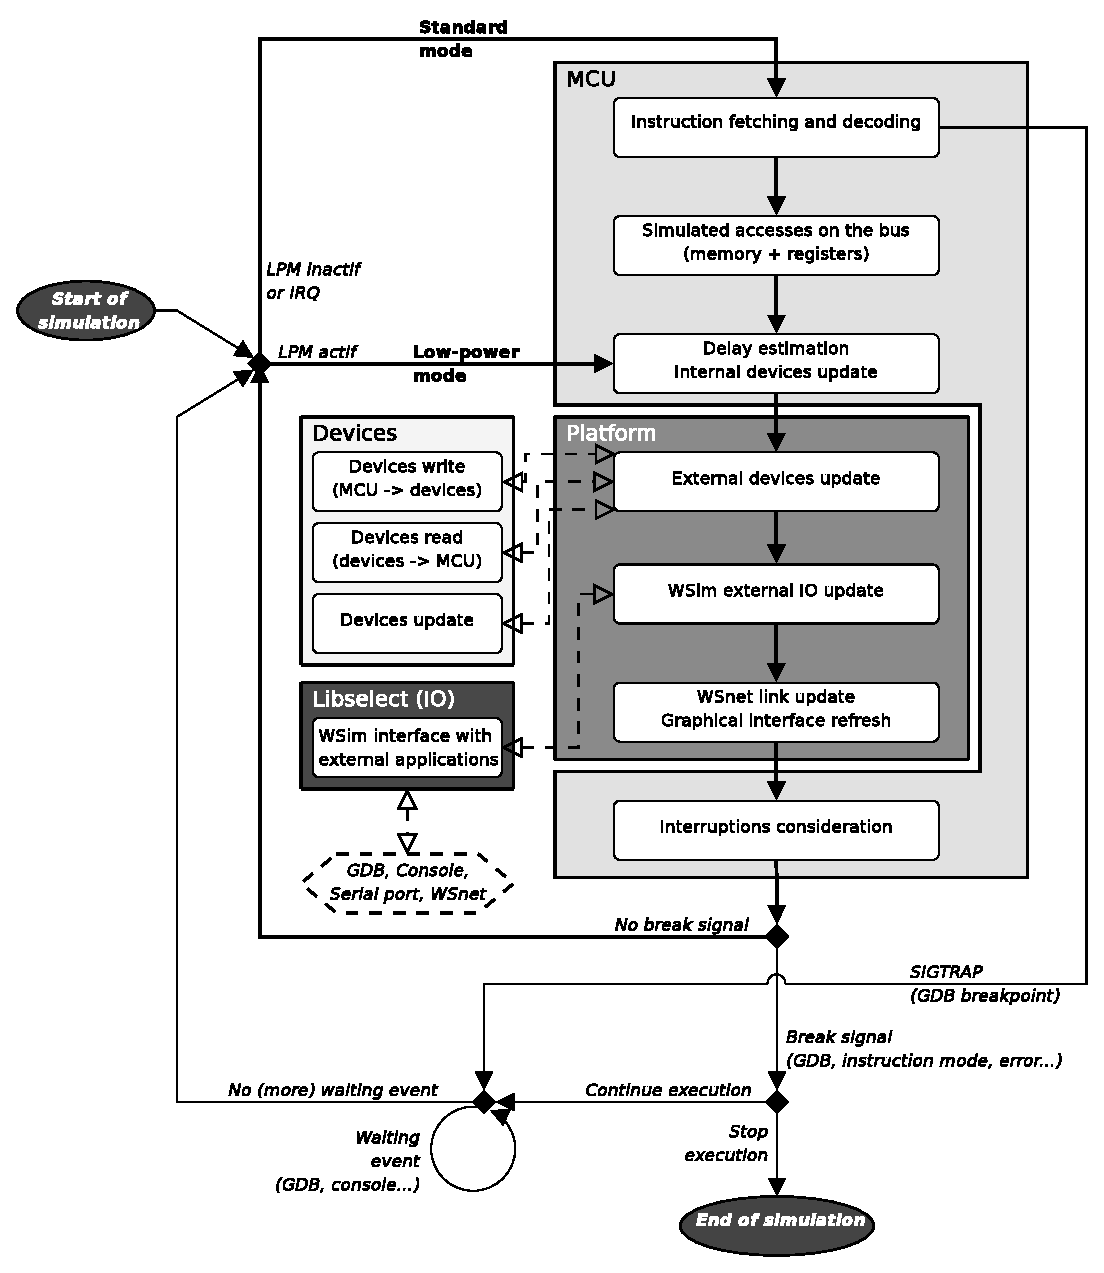
\includegraphics[scale=0.8]{figures/wsim_diag_execution.eps}
\end{center}
\caption{Steps of one instruction execution}
\label{wsim-instruction}
\end{figure}

The core of the instruction execution is the \verb$msp430_mcu_run_insn()$ function of the\\ \verb$/arch/msp430/msp430_alu.c$ file. This function fetches, decodes, executes one instruction, launches devices update and IRQ consideration (performed by \verb$msp430_mcu_update()$ function).

If the MCU is in low power mode \verb$msp430_mcu_run_lpm()$ of the \verb$/arch/msp430/msp430_alu.c$ file is called instead of \verb$msp430_mcu_run_insn()$.\\

Next paragraph describes the called functions chains, for each WSim mode, to get from the \verb$main.c$ file to the execution of one instruction.
\begin{itemize}
  \item Standard run: \verb$machine_run_free()$ $\longrightarrow$ \verb$machine_run()$ $\longrightarrow$ \verb$mcu_run()$ $\longrightarrow$ \verb$msp430_mcu_run_insn()$ or \verb$msp430_mcu_run_lpm()$ $\longrightarrow$ \verb$msp430_mcu_update()$;
  \item Instruction mode: \verb$machine_run_insn()$ $\longrightarrow$ \verb$machine_run()$ $\longrightarrow$ \verb$mcu_run()$ $\longrightarrow$ \\\verb$msp430_mcu_run_insn()$ or \verb$msp430_mcu_run_lpm()$ $\longrightarrow$ \verb$msp430_mcu_update()$;
  \item Time mode: \verb$machine_run_time$ $\longrightarrow$ \verb$machine_run()$ $\longrightarrow$ \verb$mcu_run()$ $\longrightarrow$ \verb$msp430_mcu_run_insn()$ or \verb$msp430_mcu_run_lpm()$ $\longrightarrow$ \verb$msp430_mcu_update()$;
  \item GDB mode: \verb$libgdb_target_mode_main()$ $\longrightarrow$ \verb$gdbremote_getcmd()$ $\longrightarrow$ \verb$gdbremote_single_step()$ or \verb$gdbremote_continue()$ $\longrightarrow$ \verb$machine_run_free()$ $\longrightarrow$ \verb$machine_run()$ $\longrightarrow$ \verb$mcu_run()$ $\longrightarrow$\\ \verb$msp430_mcu_run_insn()$ or \verb$msp430_mcu_run_lpm()$ $\longrightarrow$ \verb$msp430_mcu_update()$;
  \item Console mode: \verb$console_mode_main()$ $\longrightarrow$ \verb$console_command()$, then WSim starts one of the four previous mode, depending of the text string you enter on the command line.
\end{itemize}

\section{End of the simulation}
The simulation normally ends if one of these cases is true:
\begin{itemize}
  \item the \verb$*.elf$ program is finished;
  \item an illegal instruction has been detected in the \verb$*.elf$ program;
  \item the exact number of instructions has been executed (only in instruction mode);
  \item the simulation time is over (only in time mode);
  \item "quit" command has been typed (only in console mode);
  \item GBD is closed before the end of the simulation (only in GDB mode).
\end{itemize}

For standard, instruction and time modes, statistics of the simulation are written in the wsim.log file just before leaving WSim. These statistics are general informations about WSim, and more specific about machine, MCU and devices.


\chapter{Main internal features management}

\section{Memory}
\subsection{General}
Main storage are MCU state, platform external devices state (radio, leds, ...), and possibly internal platform state. A backup of these states is periodically carried out so that it allows to recover easily the previous saved state of the platform in order to backtrack.

\subsubsection{Devices and platform}
When a platform is built, an instance of each of its devices is created in order to save its states. The memory allocation  is done by the \verb$devices_memory_allocate()$ function of the \verb$devices.c$ file, located in the \verb$/devices$ directory. This function is called by the platform description file. In this function, the needed space to save the states of every platform device is computed, in order to store all the data in a contiguous memory spaces.  The pointers to access to them are stored into the \verb$machine.devices_state$ and the \verb$machine.devices_state_backup$ (\verb$machine$ is a global structure storing devices states, devices number, devices size and time of simulation).\\

Moreover saving internal platform states may be necessary. They are then stored in a platform specific structure (of your platform file), you have to define. This structure must be saved in the same contiguous space than the devices, by considering it as a device.

\subsubsection{MCU}
The MCU state and its backup are stored into global structures (\verb$mcu$ and \verb$mcu_backup$), since we know the needed space and as there is only one MCU by platform. So we need not indirections (through pointers) to access to the MCU structure, in spite of the device structure.

\subsection{Backtracks}
Backtracks are used when WSim operates with WSnet. WSim may need to backtrack in two different cases indeed:
\begin{itemize}
  \item when an event is added before next rendez-vous, and a node is running beyond this event time. An other meeting point is then set at event time, and the state of the node is restored to the last state saved.
  \item when one of WSim nodes is in debugging mode, and stopped at a breakpoint, the other nodes are still running. As soon as the WSim node in debugging mode is running again, the other nodes are backtracked.
\end{itemize}

\begin{figure}
\begin{center}
  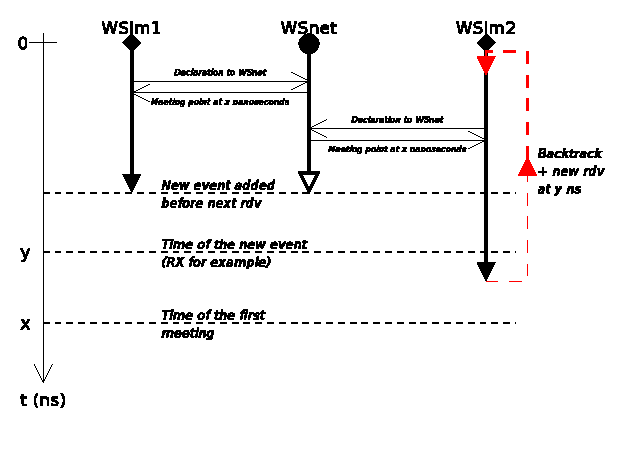
\includegraphics[scale=1]{figures/wsim_backtrack1.eps}
\end{center}
\caption{WSim backtrack when a new event is added before next rendez-vous}
\label{wsim backtrack 1}
\end{figure}

\begin{figure}
\begin{center}
  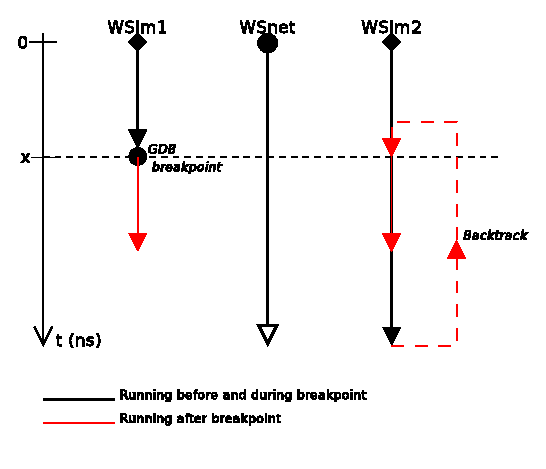
\includegraphics[scale=1]{figures/wsim_backtrack2.eps}
\end{center}
\caption{WSim backtrack in debugging mode}
\label{wsim backtrack 2}
\end{figure}

State backup saves are performed by WSim nodes through the \verb$void machine_state_save()$ function, as soon as a synchronisation is successfull or a response is received by WSnet from a WSim node. To come back from the present state to the backup one, \verb$void machine_state_restore()$ of the \verb$/machine/machine.c$ file is called. This function executes the following tasks:
\begin{itemize}
  \item restoring the state of the MCU (copy of the MCU structure in the MCU backup structure)
  \item setting the time simulation to the time of the backup
  \item replacing the content of the present state memory by the content of the backup state one
  \item restoring traces
  \item restoring WSnet state
\end{itemize}


\section{Clocks}

MSP430 time resolution is implemented in nanoseconds in WSim. Each time an instruction is executed, the MCLK is incremented and ACLK, ACLKn, SMCLK are computed according to MCLK value.\\

MSP430 clocks functions are written in the \verb$/arch/msp430/msp430_basic_clock.c$ or\\ \verb$/arch/msp430/msp430_fll_clock.c$ depending of the MSP430 model.\\

The figure \ref{wsim-clocks} presents the clocks update chain.

\begin{figure}[!h]
\begin{center}
  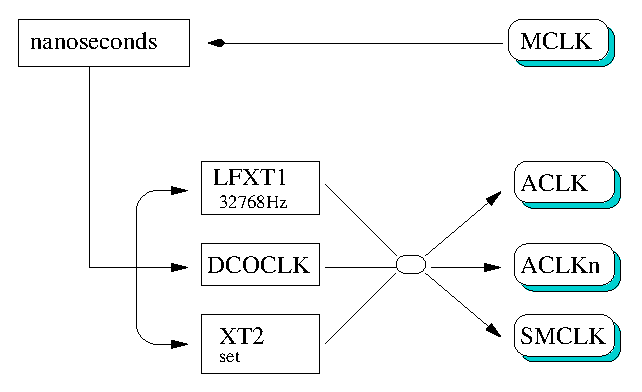
\includegraphics[scale=0.9]{figures/wsim_clocks.eps}
\end{center}
\caption{WSim MSP430 clocks design}
\label{wsim-clocks}
\end{figure}

%%%%%%%%%%%%%%%A COMPRENDRE ET AJOUTER%%%%%%%%%%%%%%%%%%%%%
%-Correspond aux é ́ché ́ances du traitement des interruptions
%-Ecriture des modèles de p ́ériph ́ériques en consé ́quences
%%%%%%%%%%%%%%%%%%%%%%%%%%%%%%%%%%%%%%%%%%%%%%%%%%%%%%%%%%%



\section{Signals}
Signals allows to signal switches of system states or errors on the *elf program execution. Two main types of signals are implemented:
\begin{itemize}
  \item The MCU internal signals
  \item The signal source identifiers
\end{itemize}


\subsection{Signals values and usages}

In the \verb$/arch/common/mcu.h$ file you can find this following code with its comments:

\begin{verbatim}
 MCU signals
  ===========

  mcu signal is a 32 bits variable that holds signal and 
  control bitfields

 
   .... .... | .... .... | .... .... | XXXX XXXX  : SIG_MCU_xxxx or HOST_SIGNAL
   .... .... | .... .... | .... ...X | .... ....  : SIG_MCU_LPM_CHANGE
  
   .... .... | .... ...X | .... .... | .... ....  : SIG_MCU          (set if SIG_MCU)
   .... .... | .... ..X. | .... .... | .... ....  : SIG_RUN_INSN     (insn single step mode)
   .... .... | .... .X.. | .... .... | .... ....  : SIG_RUN_TIME     (time single step mode)
   .... .... | .... X... | .... .... | .... ....  : SIG_GDB_SINGLE   (gdb  single step mode)
   .... .... | ...X .... | .... .... | .... ....  : SIG_GDB_IO       (IO TCP/GDB)
   .... .... | ..X. .... | .... .... | .... ....  : SIG_CON_IO       (IO Console)
   .... .... | .X.. .... | .... .... | .... ....  : SIG_WORLDSENS_IO (IO UDB/WSNnet)
   .... .... | X... .... | .... .... | .... ....  : SIG_UI           (IO UI)
  
   .... ...X | .... .... | .... .... | .... ....  : SIG_HOST         (Host signal on WSim)
   .... ..X. | .... .... | .... .... | .... ....  : SIG_MAC          (Memory access control)
   XXXX X... | .... .... | .... .... | .... ....  : SIG_MAC_xxxx


   SIG_MCU 8bits can be set either for an internal MCU signal (identified by the SIG_MCU bit)
   or for an external Unix signal on the WSim process (identified by SIG_HOST bit).

**********************************************************************************************/


/* mcu internal signal id */
#define SIG_MCU_HUP        0x00000001
#define SIG_MCU_INT        0x00000002
#define SIG_MCU_QUIT       0x00000004 /* used */
#define SIG_MCU_ILL        0x00000008 /* used */
#define SIG_MCU_TRAP       0x00000010 /* used */
#define SIG_MCU_ABRT       0x00000020
#define SIG_MCU_BUS        0x00000040 /* used */
#define SIG_MCU_TSTP       0x00000080
#define SIG_MCU_LPM_CHANGE 0x00000100
#define SIG_MCU_ALL        0x000001ff

#define SIG_HOST_SIGNAL    0x000000ff

/* signal source identifier */
#define SIG_MCU            0x00010000 /* mcu internal signal     */
#define SIG_RUN_INSN       0x00020000 /* insn mode               */
#define SIG_RUN_TIME       0x00040000 /* time mode               */
#define SIG_GDB_SINGLE     0x00080000 /* simul trap for GDB      */

#define SIG_GDB_IO         0x00100000 /* gdb tcp io request      */
#define SIG_CON_IO         0x00200000 /* console mode            */
#define SIG_WORLDSENS_IO   0x00400000 /* worldsens network io    */
#define SIG_UI             0x00800000 /* ui signal (keyboard)    */
#define SIG_HOST           0x01000000 /* host signal             */
#define SIG_MAC            0x02000000 /* mem breakpoint          */
#define SIG_BREAK_MEM_XX   0xf0000000 /*                 
\end{verbatim}

This code defines signals values.

Table \ref{mcu-signals} describes values and usages of MCU internal signals.
\begin{table}[!h]
    \begin{center}
    \begin{tabular}{|l|c|l|c|}
    \hline
      \rowcolor[gray]{0.9} \textbf{Signal} & \textbf{Value} & \textbf{Usage} & \textbf{Status} \\
    \hline
      \verb$SIG_MCU_HUP$ & \verb$0x00000001$ & Disconnection detected on the control terminal or & not used \\
      &  & death of the control processus & \\
    \hline
      \verb$SIG_MCU_INT$ & \verb$0x00000002$ & Interrupt from keyboard & not used \\
    \hline
      \verb$SIG_MCU_QUIT$ & \verb$0x00000004$ & "Quit" request from keyboard & not used \\
    \hline
      \verb$SIG_MCU_ILL$ & \verb$0x00000008$ & Illegal instruction & used\\
    \hline
      \verb$SIG_MCU_TRAP$ & \verb$0x00000010$ & Breakpoint reached & used\\
    \hline
      \verb$SIG_MCU_ABRT$ & \verb$0x00000020$ & Stop signal from \verb$abort()$ function of \verb$libc$ library & not used\\
    \hline
      \verb$SIG_MCU_BUS$ & \verb$0x00000040$ & Reading or writing at an unknown or invalid memory & used \\
      &  & address & \\
    \hline
      \verb$SIG_MCU_TSTP$ & \verb$0x00000080$ & Stop requested from tty & not used\\
    \hline
      \verb$SIG_MCU_LPM_CHANGE$ & \verb$0x00000100$ & Power mode change & not used\\
    \hline
      \verb$SIG_MCU_ALL$ & \verb$0x00000200$ & ? & not used\\
    \hline
    \end{tabular}
    \end{center}
    \caption{MCU internal signals}
    \label{mcu-signals}
\end{table}


\subsection{Signals management}
Signals are added and removed by using the \verb$mcu_signal_add()$ and \verb$mcu_signal_remove()$ commands of the \verb$arch/msp430/msp430.c$ or \verb$arch/atmega/atmega128.c$ file.
Signals status are stored in the 32 bits \verb$mcu.alu.signal$ variable.



\section{I/O}
\subsection{General}
I/Os between WSim and external applications are handled dynamically by the \verb$libselect$ library. This upper layer allows for instance to create easily an I/O for a WSim device with several possibilities of interface (TCP, UDP, STDOUT, ...). Next section lists APIs supplied by \verb$libselect$ library.

\subsection{Public functions}
\begin{itemize}
  \item \verb$libselect_id_t libselect_id_create(char *name, int UNUSED flags)$ : enables to add a dynamic external I/O (from a WSim device for example), which may be of type: TCP server (\verb$tcp:s:$), TCP client (\verb$tcp:c:$), UDP (\verb$udp:$), STDIO (\verb$stdio$), STDIN (\verb$stdin$), STDOUT (\verb$stdout$), or  (\verb$create$).

  \item \verb$int libselect_id_is_valid(libselect_id_t id)$ : to check if I/O \verb$id$ is valid (i.e. created, registered and not closed).

  \item \verb$int libselect_id_close (libselect_id_t id)$ : closes I/O \verb$id$ (deletes it of opened I/O list).

  \item \verb$int libselect_id_register(int id)$ : makes I/O \verb$id$ available.

  \item \verb$int libselect_id_unregister(int id)$ : makes I/O \verb$id$ unavailable.

  \item \verb$int libselect_id_add_callback(int id, libselect_callback callback, void *ptr)$ : function to be called if fifo of the I/O has been closed (only available for TCP I/O).

  \item \verb$uint32_t libselect_id_read(libselect_id_t id, uint8_t *data, uint32_t size)$ : gets data from the I/O fifo.

  \item \verb$uint32_t libselect_id_write(libselect_id_t id, uint8_t *data, uint32_t size)$ : puts data into the I/O fifo.

  \item \verb$int libselect_fd_register(int fd, unsigned int signal)$ : registers a file descriptor for an I/O, but just handles with its signals and reports if data is waiting in its file descriptor.

  \item \verb$int libselect_fd_unregister(int fd)$ : unregisters the file descriptor of the I/O \verb$id$.
\end{itemize}

You may refer to \verb$/devices/ptty/ptty_dev.c$, where some of these functions are used to manage the I/O of the PTTY and to section \ref{PTTY} page \pageref{PTTY} for more informations on the PTTY.


\chapter{Implementing new WSim modules}

\section{Platform}
In the WSim design, the platform file is aimed to describe it, but also to make a link between MCU and devices.
\subsection{Implementing your platform}
\subsubsection{Headers to include}
You have to include the following files in your platform implementation:
\begin{itemize}
  \item The MCU common header (\verb$#include "arch/common/hardware.h"$) and the MCU specific header (\verb$#include "arch/msp430/msp430.h"$ or \verb$#include "arch/atmega/atmega128.h"$);
  \item The device common header (\verb$#include "devices/devices.h"$) and the header of each implemented devices of the platform;
  \item \verb$#include "src/options.h"$ if you want to add platform specific options.
\end{itemize}

\subsubsection{List of mandatory functions to implement}
\begin{itemize}
  \item \verb$int devices_options_add(void)$: adds platform specific options with the \verb$option_add()$ function;
  \item \verb$int devices_create(void)$: computes the needed memory space for devices and initialise them;
  \item \verb$int devices_reset_post(void)$: function called after devices reset, so devices init conditions must be written here;	
  \item \verb$int devices_update(void)$: function called after every MCU instruction execution, this function handles input and output between MCU and devices ports.
\end{itemize}

\subsubsection{Intructions in devices\_create() function}
This function is called only once at the simulation initialisation. This intructions sequence should be followed:
\begin{enumerate}
  \item You have first to take into consideration potential specific options, that might have been provided as a command line argument (only if you implement specific option in \verb$devices_option_add()$). This is done by checking the \verb$value$ item of each option structure.
  \item MCU must be initialised by calling its \verb$MCUNAME_create()$ function;
  \item Fix each device size and store it in the \verb$machine.device_size$ table. Now call the \\ \verb$devices_memory_allocate()$ function of the \verb$/devices/devices.c$ file;
  \item Create each device with its \verb$DEVICENAME_device_create()$ function;
  \item Initialise UIs by getting their sizes (\verb$machine.device[DEVICEID].ui_get_id()$) and set their positions (\verb$machine.device[DEVICEID].ui_set_pos()$).
\end{enumerate}

\subsubsection{Intructions in devices\_update() function}
\label{platform-update}
This function is the core of the platform because it describes GPIO and SPI connections between MCU and . Thus every time the MCU decodes an intruction, this function will be called.
Instructions sequence is important and you have to follow this order as explained previously (cf chapter \ref{prog-exec} page \pageref{prog-exec}): MCU to devices transfer, devices to MCU transfer, devices update. Otherwise SPI communications might experience dysfunctions.

\begin{enumerate}
  \item First you begin by reading the MCU pins with this function: \verb$MCUNAME_digiIO_dev_read()$, that reads the 8 pins of a MCU port. Then depending of the devices pins configuration, transfer the received value on the right devices pins, by using \verb$machine.device[DEVICEID].write()$. Reiterate the sequence as many times as the number of MCU ports;
  \item Do the same operation with the UART or/and SPI ports: use \verb$msp430_UARTORSPI+ID_dev_read_$\linebreak\verb$UARTORSPI()$ to get pins value and \verb$machine.device[DEVICEID].write()$ to send it to the connected device;
  \item Now repeat the two first steps in the opposite direction, that is to say from devices to MCU pins. Use  \verb$machine.device[DEVICEID].read()$ to read devices pins and \verb$msp430_usart+ID_dev_write_$\linebreak\verb$UARTORSPI()$ to write MCU SPI or UART pins, or \verb$msp430_digiIO_dev_write()$ to write MCU GPIOs.
  \item Finally these modules must be updated:
  \begin{description}
    \item -libselect to update external I/O of WSim: \verb$LIBSELECT_UPDATE()$;
    \item -libwsnet to update link with WSnet : \verb$LIBWSNET_UPDATE()$;
    \item -platform devices to update their internal states: \verb$machine.device[DEVICEID].update()$ for each device.
  \end{description}
\end{enumerate}

\noindent\underline{Remark:} To make your platform more reliable, and give value-added to the simulation, you may add tests for illegal operations not to happen, for example:
\begin{itemize}
  \item Checking if MCU is in SPI mode before reading a SPI device;
  \item Checking if MCU is in UART mode before reading an UART device;
  \item If there are more than one device on one SPI, checking that their CSs are not enabled at the same time;
  \item Any other test you need...
\end{itemize}


\subsubsection{SDL/UI}
\label{SDL-UI}
If your platform embeds graphical device, you have to update and refresh them when required. See the leds example:
\begin{verbatim}
  /* port 5 :                          */
  /* ========                          */
  /*   P5.7 NC                         */
  /*   P5.6 led 3 (Blue)               */
  /*   P5.5 led 2 (Green)              */
  /*   P5.4 led 1 (Red)                */
  /*   P5.3 SPI flash ram UCLK         */
  /*   P5.2 SPI flash ram SOMI         */
  /*   P5.1 SPI flash ram SIMO         */
  /*   P5.0 NC                         */
  if (msp430_digiIO_dev_read(PORT5,&val8))
    {
      machine.device[LED1].write(LED1,LED_DATA, ! BIT(val8,4));
      etracer_slot_access(0x0, 1, ETRACER_ACCESS_WRITE, ETRACER_ACCESS_BIT, ETRACER_ACCESS_LVL_GPIO, 0);
      UPDATE(LED1);
      REFRESH(LED1);

      machine.device[LED2].write(LED2,LED_DATA, !  BIT(val8,5));
      etracer_slot_access(0x0, 1, ETRACER_ACCESS_WRITE, ETRACER_ACCESS_BIT, ETRACER_ACCESS_LVL_GPIO, 0);
      UPDATE(LED2);
      REFRESH(LED2);

      machine.device[LED3].write(LED3,LED_DATA, ! BIT(val8,6));
      etracer_slot_access(0x0, 1, ETRACER_ACCESS_WRITE, ETRACER_ACCESS_BIT, ETRACER_ACCESS_LVL_GPIO, 0);
      UPDATE(LED3);
      REFRESH(LED3);
    }
\end{verbatim}
On WSN430 platform leds are connected on pins 5.4, 5.5 and 5.6 of the MSP430, and are refreshed as soon as one of port 5 has been updated.

WSim also enables you to print on screen an image associated to your platform. This module is considered as a device, and is thus implemented in the \verb$/devices/uigfx$ folder. Its creation is follow the same procedure as the other devices one (\verb$uigfx_device_size()$ and \verb$uigfx_device_create()$ function).

For both devices UI and screen image, you must set the place of the graphical interface after creation. Use the device APIs \verb$machine.device[DEVICEID].ui_get_pos()$ and \verb$machine.device[DEVICEID].ui_set_pos()$ to perform this.\\

Finally if there are one or several graphical UI, the \verb$ui_refresh()$ function of the \verb$/libgui/ui.c$ file has to be called at the end of the \verb$devices_update()$ function. \verb$libgui$ module implementation relies on SDL (Simple Direct media Layer) that is a free and open source software multimedia library.


\subsection{Making your platform compilable and executable}
\label{platform-compilation}
To compile WSim, makefiles are generated with the help of the GNU Project Autotools \footnote{For further informations please see \href{http://www.gnu.org/software/automake/}{http://www.gnu.org/software/automake/} and 
\href{http://www.gnu.org/software/autoconf/}{http://www.gnu.org/software/autoconf/} websites} (automake $\ge$ 1.10, autoconf $\ge$ 2.61).
You have to modify three files to compile your platform : \verb$./configure.ac$, \verb$./platforms/Makefile.am$, \verb$./platforms/YOURPLATFORMFOLDER/Makefile.am$.

\subsubsection{/configure.ac}
\begin{enumerate}
  \item In the \verb$platform model$ part, add an option to enable to compile only your platform by using the command \verb$./configure --enable-platform-yourplatformname$:
\begin{verbatim}
dnl yourplatformname
AC_ARG_ENABLE([platform-yourplatformname],AS_HELP_STRING([--enable-\
platform-yourplatformname],[yourplatformname platform]))
if test "${enable_platform_senslab}" = "yes" ; then
	enable_mcu_msp430=yes  dnl or enable_mcu_atmega=yes
	NPLATFORM=$(($NPLATFORM + 1))
	PLATFORMNAMES="yourplatformname"
fi
\end{verbatim}

  \item And at the end of the \verb$platform model$ part insert the following line:
\begin{verbatim}
AM_CONDITIONAL([BUILD_YOURPLATFORMNAME],   [test "${enable_platform_yourplatformname}"   \
= "yes" -o "$ALL" = "yes" ])
\end{verbatim}
This line initialises the \verb$BUILD_YOURPLATFORMNAME$ variable to \verb$1$ if your platform only or all the platforms must be built, else to \verb$0$ (the purpose of this variable is developed in paragraph \ref{yourplatformmakefile} page \pageref{yourplatformmakefile}).\\

  \item Add the path to your platform makefile into \verb$AC_CONFIG_FILES$ of the output part: 
\begin{verbatim}
platforms/YOURPLATFORMFOLDER/Makefile
\end{verbatim}
\end{enumerate}

\subsubsection{/platforms/Makefile.am}
Simply add the name of your platform directory in the \verb$SUBDIRS$ variable.
\begin{verbatim}
SUBDIRS=wsn430 ot2006 otsetre ez430 tests telosb \
	mosar mica2 micaz iclbsn wisenode senslab yourplatformname
\end{verbatim}

\subsubsection{/platforms/YOURPLATFORMFOLDER/Makefile.am}
\label{yourplatformmakefile}
\begin{enumerate}
  \item First test if your platform must be built or not, thanks to the \verb$BUILD_YOURPLATFORMNAME$ variable defined with the \verb$AM_CONDITIONAL$ command in the \verb$configure.ac$ file: 
\begin{verbatim}
if BUILD_YOURPLATFORMNAME
\end{verbatim}

 \item  Next set the program name and the worldsens program name (program running with WSnet) for your platform:
\begin{verbatim}
bin_PROGRAMS=wsim-yourplatformname
if BUILD_WORLDSENS
bin_PROGRAMS+=worldsens-yourplatformname
endif
\end{verbatim}

  \item This line adds preprocessor arguments (here it enables to include /wsim top directory at compilation):
\begin{verbatim}
INCLUDES=-I$(top_srcdir)
\end{verbatim}

  \item Then define the MCU and devices libraries dependencies paths. For instance:
\begin{verbatim}
YOURPLATFORMNAME_MCU= ../../arch/msp430/libmsp430f1611.a
YOURPLATFORMNAME_DEV= ../../devices/led/libled.a        \
                      ../../devices/ds2411/libds2411.a  \
                      ../../devices/m25p80/libm25p80.a  \
                      ../../devices/ptty/libptty.a      \
                      ../../devices/uigfx/libuigfx.a    \
                      ../../devices/cc1100/libcc1100.a
\end{verbatim}

  \item Add specific compilation flags:
\begin{verbatim}
wsim_yourplatformname_CFLAGS=-DMSP430f1611
\end{verbatim}
This flag will define the global macro MSP430f1611 during the compilation.

  \item Declare the name of your platform source file:
\begin{verbatim}
wsim_yourplatformname_SOURCES=yourplatformname.c
\end{verbatim}

  \item Declare the libraries dependencies path set below: 
\begin{verbatim}
wsim_yourplatformname_LDADD=${YOURPLATFORMNAME_DEV} ${WSIMADD} ${YOURPLATFORMNAME_MCU}
\end{verbatim}
\verb!${WSIMADD}! is defined in the \verb$/platform/Makefile.am$ file, and sets some general WSim library dependence.

  \item  Finally do not forget to close the \verb$if BUILD_YOURPLATFORMNAME$
\begin{verbatim}
endif
\end{verbatim}

\end{enumerate}

\section{Device}
\subsection[Adding a new device model]{Adding a new device model\protect\footnote{Templates sources codes are available in appendix \ref{spi-device-template} page \pageref{spi-device-template}}} 
\label{adding-device}
\subsubsection{List of mandatory APIs to implement}
\begin{itemize}
  \item \verb$int YOURDEVICENAME_add_options()$: enables to add device specific options when starting a simulation.
  \item \verb$int YOURDEVICENAME_device_size()$: returns size the device structure needs to store its internal states.
  \item \verb$int YOURDEVICENAME_device_create()$: creates an instance of the device, by initialising the states in \verb$machine.device[DEVICEID].data$ and storing in \verb$machine.device[DEVICEID]$ device private functions to be called during the simulation.
\end{itemize}


\subsubsection{List of private functions to implement}
Depending of devices features some of these private functions have to be implemented:
\begin{itemize}
  \item \verb$int YOURDEVICENAME_write()$: transmits MCU informations to the device
  \item \verb$int YOURDEVICENAME_read()$: transmits device informations to the MCU (for example leds need not this function);
  \item \verb$int YOURDEVICENAME_update()$: updates internal state of the device after read or write action (for instance emptying radio TX buffer after its content has been transmitted to the MCU);
  \item \verb$int YOURDEVICENAME_delete()$: frees memory space filled by the device (excepted the device states);
  \item \verb$int YOURDEVICENAME_reset()$: resets the device (at its default states);
  \item \verb$int YOURDEVICENAME_power_up()$: for potential future use;
  \item \verb$int YOURDEVICENAME_power_down()$: for potential future use;
  \item \verb$int YOURDEVICENAME_ui_draw()$: draws device graphical interface;
  \item \verb$int YOURDEVICENAME_ui_set_pos()$: sets the position of device graphical interface;
  \item \verb$int YOURDEVICENAME_ui_get_pos()$: gives the position of device graphical interface;
  \item \verb$int YOURDEVICENAME_ui_get_size()$: gives the size of device graphical interface;
  \item \verb$int YOURDEVICENAME_statdump()$: may be used to return device statistics (called only at the end of the simulation).
\end{itemize}


\subsubsection{device\_t structure}
\verb$device_t$ structure stores function addresses described in the previous subsection, in order to make their calls easier. The structure is designed like this:
\begin{verbatim}
struct device_t
{
  int  (*update)        (int self);
  void (*read)          (int self, uint32_t *mask, uint32_t *value);
  void (*write)         (int self, uint32_t  mask, uint32_t  value);

  // create is static
  // size   is static
  int  (*delete)        (int self);

  int  (*reset)         (int self);
  int  (*power_up)      (int self);
  int  (*power_down)    (int self);

  int  (*ui_draw)       (int self);
  void (*ui_set_pos)    (int self, int  x, int  y);
  void (*ui_get_pos)    (int self, int *x, int *y);
  void (*ui_get_size)   (int self, int *width, int *height);

  void (*statdump)      (int self, int64_t user_nanotime);

  int state_size;
  int dev_num;

  char* name;
  void* data;
};
\end{verbatim}
Of course using all items of the structure is not mandatory.

\subsubsection{LED example}
LED device is the simplest example of device implementation. Only \verb$write()$, \verb$delete()$, \verb$reset()$, and graphical functions are used in the list of \verb$device_t$ private functions.
However its \verb$create()$ function is closed to the other devices ones. It mainly consists in storing private functions addresses in the \verb$machine.device[DEVICEID]$ structure.
\begin{verbatim}
int led_device_create(int dev_num, uint32_t on, uint32_t off, uint32_t bg, char* name)
{
  struct led_t *dev = (struct led_t*) machine.device[dev_num].data;
  
  dev->img      = led_img_create(on,off,bg);
  dev->update   = 0;
  dev->val      = 0;
  dev->trid     = tracer_event_add_id(1, name, "led");

  machine.device[dev_num].reset         = led_reset;
  machine.device[dev_num].delete        = led_delete;

  machine.device[dev_num].write         = led_write;
  machine.device[dev_num].update        = led_update;

  machine.device[dev_num].ui_draw       = led_ui_draw;
  machine.device[dev_num].ui_get_size   = led_ui_get_size;
  machine.device[dev_num].ui_set_pos    = led_ui_set_pos;
  machine.device[dev_num].ui_get_pos    = led_ui_get_pos;

  machine.device[dev_num].state_size    = led_device_size();
  machine.device[dev_num].name          = "Led display";

  return 0;
}
\end{verbatim}


\subsection{IO pins interface management}
\subsubsection{General}
There are 2 main class of IO, GPIOs for general use, and USART. IO device pins are the interface between device and MCU. In the platform file, these pins are going to be read and write from/to MCU, thanks to read and write device functions as described below. To select the device pin to read or write, a mask variable may be used. For example, the following masks are defined for the M25P80 flash memory device (in the \verb$./devices/m25p80/m25p80.h$ file):

\begin{verbatim}
#define M25P_W_SHIFT  8 /* write protect */
#define M25P_S_SHIFT  9 /* select        */
#define M25P_H_SHIFT 10 /* hold          */
#define M25P_C_SHIFT 11 /* clock         */

#define M25P_D  0x00ff               /** data 8 bits           **/
#define M25P_W  (1 << M25P_W_SHIFT)  /** write protect negated **/
#define M25P_S  (1 << M25P_S_SHIFT)  /** chip select negated   **/
#define M25P_H  (1 << M25P_H_SHIFT)  /** hold negated          **/
#define M25P_C  (1 << M25P_C_SHIFT)  /** clock                 **/
\end{verbatim}

\medskip
Table \ref{m25p80-masks} and figure \ref{wsim-m25p80} clarifies this C code:

\begin{table}[!h]
  \begin{minipage}[b]{0.50\linewidth}
    \begin{center}
    \begin{tabular}{|l|l|l|}
    \hline
      \rowcolor[gray]{0.9} \textbf{Name} & \textbf{Value} & \textbf{Pin(s)} \\
    \hline
      \verb$M25P_D$ & \verb$0000 0000 1111 1111$ & \verb$SPI SDI, SPI SDO$ \\
    \hline
      \verb$M25P_W$ & \verb$0000 0001 0000 0000$ & \verb$FLASH W$ \\
    \hline
      \verb$M25P_S$ & \verb$0000 0010 0000 0000$ & \verb$FLASH CS$ \\
    \hline
      \verb$M25P_H$ & \verb$0000 0100 0000 0000$ & \verb$FLASH HOLD$ \\
    \hline
      \verb$M25P_C$ & \verb$0000 1000 0000 0000$ & \verb$SPI CLOCK$ \\
    \hline
    \end{tabular}
    \end{center}
    \caption{Value of the M25P80 masks}
    \label{m25p80-masks}
  \end{minipage}\hfill
    \begin{minipage}[b]{0.40\linewidth}
    \begin{center}
      \centering 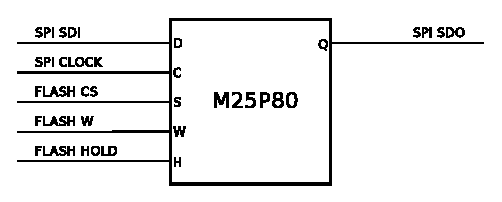
\includegraphics[scale=0.8]{figures/wsim_m25p80.eps}
    \end{center}
    \caption{M25P80 pins configuration}
    \label{wsim-m25p80}
  \end{minipage}
\end{table}

\medskip
Thus, writing CS and HOLD pins might be implement like this:
\begin{verbatim}
uint32_t value = 0000 0110 0000 0000;
machine.device[FLASH].write(FLASH, M25P_H | M25P_S, value);
\end{verbatim}

\subsubsection{USART}
On the MSP430, USART may be configured in three modes: SPI, UART and I2C. However I2C is not implemented in WSim yet.\\

The WSim simulation of USART does not follow exactly the real hardware running. Instead of sending data bit by bit to devices, WSim USART transmits byte by byte, in simulating the time to send one byte. Hence a byte is only ready to be transmitted after 8 UCLK cycles have been counting. The same method is used for USART data reception from devices.
It allows to simplify USART transfer implementation and to save computation time by avoiding functions calls.\\

This choice of implementation has no effects on the reliability of the simulation.


\subsubsection{SPI particularity}
SPI bus works always in full duplex, that is to say every time data is transmitted to a SPI device, this one sends a synchronized response at the same time. Thus, in order to get data from a SPI device if nothing has to be transfered to it, you must send a dummy data to trigger the device response.\\

In WSim, SPI interface is implemented in the \verb$arch/msp430/msp430_usart.c$ file for the MSP430 MCU. This implementation do not check if SPI communication are full duplex. It may be done in your platform or in your device code.\\

The better way to implement SPI full duplex communications, is to take it into consideration in your device model code. As soon as your device \verb$YOURDEVICENAME_write()$ function is called by your platform for SPI writings, data must be immediately available for \verb$YOURDEVICENAME_read()$ function.

As explained in subsection \ref{platform-update} page \pageref{platform-update}, the \verb$device_update()$ function of the platform performs writings (on devices, so readings on MCU), readings (on devices, so writings on MCU), and finally update devices.\\

However all devices models may not be implemented in that way. For some devices (cc2420, cc1100, ...), writing on their SPI input (SI) is taken into consideration only when the device is updated at the end of a updating platform cycle. As the reading action is performed after the writing one, no response is sent on the device SPI output (SO) yet.\\

This leads to a small lag between the simulation and the reality, since the SPI UxRXBUF register receives the response on the next \verb$device_update()$ call, that is to say few MCU cycles later (from 1 to 6).
The figure~\ref{wsim-spi-communication} illustrates that.\\

\begin{figure}[!h]
\begin{center}
  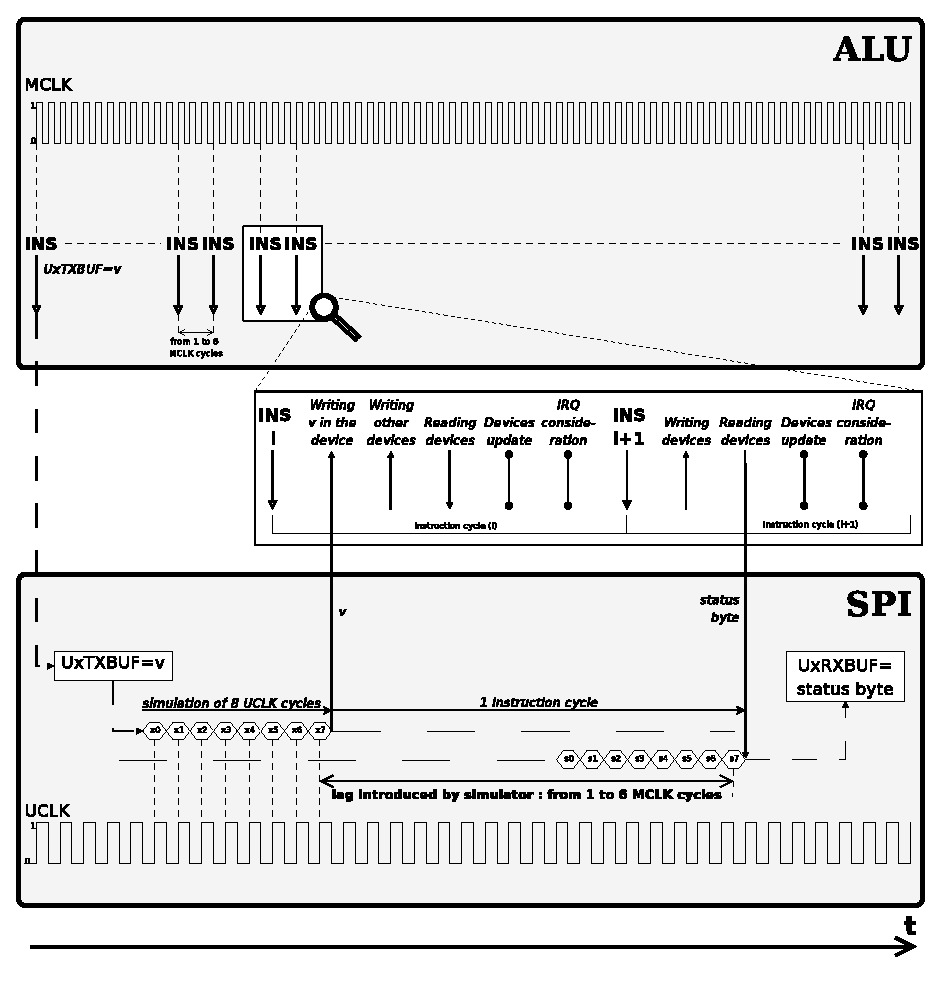
\includegraphics[scale=1]{figures/wsim_spi.eps}
\end{center}
\caption{WSim SPI and device communication particular case}
\label{wsim-spi-communication}
\end{figure}

In most cases this small lag will not be annoying.


\subsection{Making your device model compilable}
The procedure to make your device model compilable is quite similar to the platform one (please refer to the subsection \ref{platform-compilation} page \pageref{platform-compilation} for more details). Thus you have to modify these following files to compile your device : \verb$./configure.ac$, \verb$./devices/Makefile.am$, \verb$./devices/YOURDEVICEFOLDER/Makefile.am$.

\subsubsection{/configure.ac}
Add the path to your device makefile into \verb$AC_CONFIG_FILES$ of the output part: 
\begin{verbatim}
devices/YOURDEVICEFOLDER/Makefile
\end{verbatim}

\subsubsection{/devices/Makefile.am}
Simply add the name of your platform directory in the \verb$SUBDIRS$ variable.
\begin{verbatim}
SUBDIRS =   \
    7seg    \
    at45db  \
    bargraph\
    cc1100  \
    cc2420  \
    ds2411  \
    gdm1602a\
    hd44780 \
    led     \
    m25p80  \
    ptty    \
    uigfx   \
    yourdevicename
\end{verbatim}

\subsubsection{/devices/YOURDEVICEFOLDER/Makefile.am}
Compilation of your device model source has to build a static library \verb$*.a$, to make it reusable.
\begin{enumerate}
  \item First set the name of your device library and require it not be installed:
\begin{verbatim}
noinst_LIBRARIES=libyourdevicename.a
\end{verbatim}

  \item Next add this line to give additional preprocessor arguments (here it enables to include /wsim top directory at compilation):
\begin{verbatim}
INCLUDES=-I$(top_srcdir)
\end{verbatim}

  \item Declare the name of your device model source files, for example:
\begin{verbatim}
libled_a_SOURCES=yourdevicename_source1.h yourdevicename_source1.c\
                 yourdevicename_source2.h yourdevicename_source2.c\
                 yourdevicename_source3.h yourdevicename_source4.h\
\end{verbatim}

\end{enumerate}

\section{Special device}

We may distinguish 2 special devices: the pseudo serial PTTY and the graphical interface for platform UIGFX. They are special in the meaning that they do not stand for a hardware component. Nevertheless their implementation is quite the same as a standard device, especially their API functions (please see section \ref{adding-device} page \pageref{adding-device} for more details). They have to be initialised and updated in the platform file like other devices indeed.

\subsection{Pseudo TTY}
\label{PTTY}
The PTTY (Pseudo TTY) peripheral model is a special peripheral that can be used to connect a platform to a RS232 serial port. The model has the capability to open a full duplex communication stream with the operating system in order to connect the simulator to external tools.

\begin{figure}[!h]
\begin{center}
  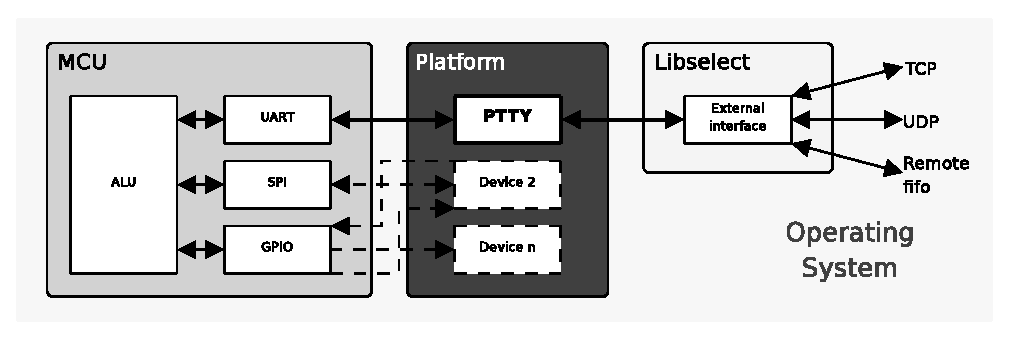
\includegraphics[scale=1]{figures/wsim_ptty.eps}
\end{center}
\caption{WSim PTTY device integration}
\label{wsim-ptty}
\end{figure}

The PTTY mainly makes the link between the platform and \verb$libselect$ functionalities.
\begin{itemize}
  \item To send data to the OS: PTTY device calls \verb$libselect_id_write()$.
  \item To get data from the OS: PTTY device calls \verb$libselect_id_read()$.
  \item To delete the PTTY device: PTTY delete the \verb$libselect$ connection with the \verb$libselect_id_close()$ function.
\end{itemize}


These 3 additional functions are designed to avoid and handle with errors :
\begin{itemize}
  \item \verb$ptty_dummy_read()$ : sets value and mask to 0.
  \item \verb$ptty_dummy_write()$ : writes to \verb$/dev/null$.
  \item \verb$ptty_libselect_callback()$ : not used.
\end{itemize}

\subsection{Graphical interface for platform UIGFX}
Please refer to section \ref{SDL-UI} page \pageref{SDL-UI} for some further informations.


\section{Microcontroller}


\chapter{Debugging WSim}

There are several methods to debug WSim code source.

\section{wsim.log file}

At each simulation a log file is generated by WSim, named wsim.log and located in the directory where WSim has been launched. This file contains debugging information.
To enable debugging information, you have to define the macro DEBUG. There are two ways to do so:

\begin{itemize}
  \item when launching \verb$configure$ file before compiling WSim add the option \verb$./configure --enable-debug$;
  \item or define directly the macro \verb$DEBUG$ in the WSim file \verb$xxx_debug.h$ located in the same directory than the file you want to debug, as shown in the following example:
\end{itemize}

\begin{verbatim}
/**
 *  \file   cc2420_debug.h
 *  \brief  CC2420 debug messages 
 *  \author Nicolas Boulicault
 *  \date   2007
 **/

/*
 *  cc1100_debug.h
 *  
 *
 *  Created by Nicolas Boulicault on 04/06/07.
 *  Copyright 2007 __WorldSens__. All rights reserved.
 *
 */

#ifndef _CC2420_DEBUG_H_
#define _CC2420_DEBUG_H_

/***************************************************/
/***************************************************/
/***************************************************/

#define DEBUG
#if defined(DEBUG)
#define CC2420_DEBUG(x...)     VERBOSE(2,x)
#define CC2420_DBG_RX(x...)    VERBOSE(2,x)
#define CC2420_DBG_TX(x...)    VERBOSE(2,x)
#else
#define CC2420_DEBUG(x...)     do { } while (0)
#define CC2420_DBG_RX(x...)    do { } while (0)
#define CC2420_DBG_TX(x...)    do { } while (0)
#endif

/***************************************************/
/***************************************************/
/***************************************************/

#define CC2420_PINS_DEBUG

\end{verbatim}

The second method has the advantage to print only debug messages of the file where \verb$DEBUG$ is defined, contrary to the first one that behaves like \verb$DEBUG$ were defined in each file of the program.

By default, debugging information in wsim.log file is minimal.(default verbose level equal to 0). Nevertheless more information may be output be increasing verbose level when starting simulation: \verb$--verbose=6$ for instance.
In the previous code, we have \verb$#define CC2420_DBG_RX(x...)    VERBOSE(2,x)$. This means that the \verb$CC2420_DBG_RX$ will be print in the wsim.log file only if the verbose level is superior or equal to 2.

Thus you understand that it is quite easy to add your own debug informations, if you need. You just have to define the print debugging function with its verbose level at the beginning of your file (or its associated *.h file). Then insert it with appropriate debugging message (a \verb$printf()$ function) at the right place.

Note that the \verb$wsim.log$ file name may be changed into \verb$NAMEOFYOURCHOICE.log$ by using the option \verb$--logfile=NAMEOFYOURCHOICE.log$. Moreover WSim \verb$--logfile$ option also supports \verb$stdout$ and \verb$stdin$ redirection (for instance \verb$--logfile=stderr$).

\section{ERROR() function}
The \verb$ERROR()$ function is closed to the \verb$VERBOSE()$ function, excepted that its result is printed in the wsim.log file and in the standard error output too, that is to say the terminal you launch WSim.
You can insert \verb$ERROR()$ function where you want without needs to declare it. Its syntax is as a \verb$printf()$ function.
Moreover some ERROR messages are printed only if the macro \verb$DEBUG_ME_HARDER$ is defined:
\begin{verbatim}
#if defined(DEBUG_ME_HARDER)
	    ERROR("senslab:devices: read data on radio while not in SPI mode ?\n");
#endif
\end{verbatim}

\section{WSim trace}
The \verb$tracer_event_record()$ function, insered in the Wsim code, allows to save states of a variable during the simulation. To enable the trace storage, you just have to add the following option when starting a simulation: \verb$--trace$ (example: \verb$wsim-wsn430 --ui --trace --mode=time --modearg=100000000000$ \verb$wsn430-leds.elf$). The trace is then stored in the \verb$wsim.trc$ file and located in the  directory where WSim has been launched.

To make the wsim.trc file usable, you have to convert it with the external wtracer application, according to the following syntax. For instance:
\begin{itemize}
  \item\verb$wtracer --in=wsim.trc --out=wsim.gp --format=gplot$ generates the gnuplot wsim.gp file. 
  \item\verb$wtracer --in=wsim.trc --out=wsim.vcd --format=vcd$ generates the vcd wsim.vcd file, readable by GTKwave.
\end{itemize}


\section{Using GDB}
It is also possible to debug WSim by using GDB. Launch GDB in the folder where the *.elf file is located, set your breakpoints, and execute the run command followed by the WSim arguments, including your *.elf file. Here is an example:
\begin{verbatim}
loic@loic-laptop:~/Documents/Senstools/temp/senslab/node/wsn430_SW/wsn430-drivers/
wsn430-cc2420\$ gdb wsim-senslabv14
GNU gdb 6.8-debian
Copyright (C) 2008 Free Software Foundation, Inc.
License GPLv3+: GNU GPL version 3 or later <http://gnu.org/licenses/gpl.html>
This is free software: you are free to change and redistribute it.
There is NO WARRANTY, to the extent permitted by law.  Type "show copying"
and "show warranty" for details.
This GDB was configured as "i486-linux-gnu"...
(gdb) b main.c:200
Breakpoint 1 at 0x8054568: file main.c, line 200.
(gdb) r cc2420-tx.elf 
Starting program: /usr/local/bin/wsim-senslabv14 cc2420-tx.elf
[Thread debugging using libthread_db enabled]
[New Thread 0xb7c168c0 (LWP 23589)]
[Switching to Thread 0xb7c168c0 (LWP 23589)]

Breakpoint 1, main (argc=2, argv=0xbf976f24) at main.c:200
200	  options_start();
(gdb) n
201	  ui_options_add();
(gdb) 
\end{verbatim}


\chapter{Appendix}

\section{Abbreviations}
\begin{description}
  \item \textbf{ACLK} = Auxiliary Clock (of the MCU)
  \item \textbf{CS} = Chip Select
  \item \textbf{GPIO} = General Purpose Input Output
  \item \textbf{I2C} = Inter Integrated Circuit
  \item \textbf{IO} = Input Output
  \item \textbf{IRQ} = Interrupt Request
  \item \textbf{LPM} = Low Power Mode (for the MCU)
  \item \textbf{MCLK} = Master Clock (of the MCU)
  \item \textbf{MCU} = MicroController Unit
  \item \textbf{PTTY} = Pseudo Terminal Type
  \item \textbf{SI} = SPI device input
  \item \textbf{SMCLK} = Sub Main Clock (of the MCU)
  \item \textbf{SO} = SPI device output
  \item \textbf{SPI} = Serial Peripheral Interface
  \item \textbf{UART} = Universal Asynchronous Receiver Transmitter
  \item \textbf{UCLK} = Uncore Clock
  \item \textbf{UI} = User Interface
  \item \textbf{USART} = Universal Synchronous/Asynchronous Receiver Transmitter
  \item \textbf{UxRXBUF} = MSP430 SPI register used for reception
  \item \textbf{UxTXBUF} = MSP430 SPI register used for transmission
\end{description}

\section{Templates}
\subsection{SPI device}
\label{spi-device-template}

These templates are aimed to help you to develop your own SPI device model. You just have to replace \verb$spidev$ string by your device model name, and to implement the body of the functions you need. \verb$spidev_dev.c$ and \verb$spidev_dev.h$ are the minimal files to write a device model. However depending on its complexity, you may need additional files.

These source codes are also available in the \verb$/devices/spidev$ folder.

\subsubsection{spidev\_dev.c}
\begin{verbatim}

/**
 *  \file   spidev_dev.c
 *  \brief  SPI device example
 *  \author Antoine Fraboulet
 *  \date   2009
 **/

#include <stdio.h>
#include <stdlib.h>
#include <string.h>

#include "arch/common/hardware.h"
#include "devices/spidev/spidev_dev.h"
#include "src/options.h"

/***************************************************/
/***************************************************/

#define NAME      "spidev"

tracer_id_t TRACER_SPIDEV_STATE;
tracer_id_t TRACER_SPIDEV_STROBE;

/***************************************************/
/***************************************************/

#ifdef DEBUG
#define MSG_DEVICES       2
#define DEBUG_ME_HARDER
#define HW_DMSG_SPI(x...) VERBOSE(MSG_DEVICES,x)
#else
#define HW_DMSG_SPI(x...) do {} while(0)
#endif

/***************************************************/
/***************************************************/
/***************************************************/

struct spidev_t 
{

  uint8_t select_bit;           /* chip select   */
  uint8_t hold_bit;             /* hold          */
  uint8_t write_protect_bit;    /* write protect */

  /* data just written */
  uint8_t data_buffer;
  uint8_t data_buffer_ok;

  /* data to be read */
  uint8_t data_ready;
  uint8_t data_val;
  
  /* busy timing */
  uint64_t end_of_busy_time;

  /* clock pin : unused */
  uint8_t clock;
};

#define SPIDEV_DATA        ((struct spidev_t*)(machine.device[dev].data))

/***************************************************/
/** Flash external entry points ********************/
/***************************************************/

int  spidev_reset       (int dev);
int  spidev_delete      (int dev);
int  spidev_power_up    (int dev);
int  spidev_power_down  (int dev);
void spidev_read        (int dev, uint32_t *mask, uint32_t *value);
void spidev_write       (int dev, uint32_t  mask, uint32_t  value);
int  spidev_update      (int dev);
int  spidev_ui_draw     (int dev);
void spidev_ui_get_size (int dev, int *w, int *h);
void spidev_ui_set_pos  (int dev, int  x, int  y);
void spidev_ui_get_pos  (int dev, int *x, int *y);

/***************************************************/
/***************************************************/
/***************************************************/

#define MAXNAME 1024

int spidev_add_options(int UNUSED dev_num, int dev_id, const char UNUSED *dev_name)
{
  if (dev_id >= 1)
    {
      ERROR("spidev: too much devices, please rewrite option handling\n");
      return -1;
    }

  return 0;
}

/***************************************************/
/***************************************************/
/***************************************************/

int spidev_device_size()
{
  return sizeof(struct spidev_t);
}

/***************************************************/
/***************************************************/
/***************************************************/

int spidev_device_create(int dev, int UNUSED id)
{
  machine.device[dev].reset         = spidev_reset;
  machine.device[dev].delete        = spidev_delete;
  machine.device[dev].power_up      = spidev_power_up;
  machine.device[dev].power_down    = spidev_power_down;

  machine.device[dev].read          = spidev_read;
  machine.device[dev].write         = spidev_write;
  machine.device[dev].update        = spidev_update;

  machine.device[dev].ui_draw       = spidev_ui_draw;
  machine.device[dev].ui_get_size   = spidev_ui_get_size;
  machine.device[dev].ui_set_pos    = spidev_ui_set_pos;

  machine.device[dev].state_size    = spidev_device_size();
  machine.device[dev].name          = NAME " example";

#if defined(DEBUG_ME_HARDER)
  HW_DMSG_SPI(NAME ": =================================== \n");
  HW_DMSG_SPI(NAME ": 0000 CHSW dddd dddd == MASK         \n");
  HW_DMSG_SPI(NAME ":      C              : Clock         \n");
  HW_DMSG_SPI(NAME ":       M             : MiSo          \n");
  HW_DMSG_SPI(NAME ":        S            : Chip Select   \n");
  HW_DMSG_SPI(NAME ":         W           : Write Protect \n");
  HW_DMSG_SPI(NAME ":           dddd dddd : SPI data      \n");
  HW_DMSG_SPI(NAME ": =================================== \n");
#endif

  TRACER_SPIDEV_STATE  = tracer_event_add_id(8, "state"    , NAME);
  TRACER_SPIDEV_STROBE = tracer_event_add_id(8, "function" , NAME);

  return 0;
}

/***************************************************/
/***************************************************/
/***************************************************/

int spidev_reset(int UNUSED dev)
{
  HW_DMSG_SPI(NAME ": device reset\n");
  return 0;
}

/***************************************************/
/***************************************************/
/***************************************************/

int spidev_delete(int UNUSED dev)
{
  HW_DMSG_SPI(NAME ": device delete\n");
  return 0;
}

/***************************************************/
/***************************************************/
/***************************************************/

int spidev_power_up(int UNUSED dev)
{
  HW_DMSG_SPI(NAME ": device power up\n");
  return 0;
}

int spidev_power_down(int UNUSED dev)
{
  HW_DMSG_SPI(NAME ": device power down\n");
  return 0;
}

/***************************************************/
/***************************************************/
/***************************************************/

/*
 * read is done only on a junk write
 *
 */

void spidev_read(int UNUSED dev, uint32_t *mask, uint32_t *value)
{
  *mask  = 0;
  *value = 0;
  
  if (*mask != 0)
    {
      HW_DMSG_SPI(NAME ": device write to mcu [val=0x%02x,mask=0x%04x] \n", *value, *mask);
    }
}

/***************************************************/
/***************************************************/
/***************************************************/

void spidev_write(int dev, uint32_t mask, uint32_t value)
{
  HW_DMSG_SPI(NAME ": device write from mcu value 0x%04x mask 0x%04x\n",value, mask);

  /***************************
   * Control pins. WRITE PROTECT
   ***************************/

  if (mask & SPIDEV_W) /* write protect netgated */
    {
      SPIDEV_DATA->write_protect_bit  = ! (value & SPIDEV_W);
      HW_DMSG_SPI(NAME ":    flash write protect W = %d\n",SPIDEV_DATA->write_protect_bit);
    }

  /***************************
   * Control pins. CLOCK
   ***************************/

  if (mask & SPIDEV_C) /* clock */
    {
      ERROR(NAME ":    clock pin should not be used during simulation\n");
      HW_DMSG_SPI(NAME ":    clock pin should not be used during simulation\n");
      SPIDEV_DATA->clock = (value >> SPIDEV_C_SHIFT) & 0x1;
    }
}

/***************************************************/
/***************************************************/
/***************************************************/

int spidev_update(int UNUSED dev)
{
  return 0;
}

/***************************************************/
/***************************************************/
/***************************************************/

int spidev_ui_draw      (int UNUSED dev)
{
  return 0;
}

void spidev_ui_get_size (int UNUSED dev, int *w, int *h)
{
  w = 0;
  h = 0;
}

void spidev_ui_set_pos  (int UNUSED dev, int UNUSED x, int UNUSED y)
{
  
}

void spidev_ui_get_pos  (int UNUSED dev, int *x, int *y)
{
  *x = 0;
  *y = 0;
}

/***************************************************/
/***************************************************/
/***************************************************/
\end{verbatim}

\subsubsection{spidev\_dev.h}

\begin{verbatim}

/**
 *  \file   spidev_dev.h
 *  \brief  SPI device example
 *  \author Antoine Fraboulet
 *  \date   2009
 **/

#ifndef SPIDEV_DEVICES_H
#define SPIDEV_DEVICES_H

#define SPIDEV_W_SHIFT  8 /* write protect */
#define SPIDEV_S_SHIFT  9 /* select        */
#define SPIDEV_M_SHIFT 10 /* MISO          */
#define SPIDEV_C_SHIFT 11 /* clock         */

#define SPIDEV_D  0x00ff                 /** data 8 bits           **/
#define SPIDEV_W  (1 << SPIDEV_W_SHIFT)  /** write protect negated **/
#define SPIDEV_S  (1 << SPIDEV_S_SHIFT)  /** chip select negated   **/
#define SPIDEV_M  (1 << SPIDEV_M_SHIFT)  /** miso                  **/
#define SPIDEV_C  (1 << SPIDEV_C_SHIFT)  /** clock                 **/

int  spidev_add_options   (int dev_num, int dev_id, const char *name);
int  spidev_device_size   ();
int  spidev_device_create (int dev_num, int dev_id);

#endif
\end{verbatim}

\end{document}          
